\section{VEHICULOS}
\subsection{Gráfico de dependencias}
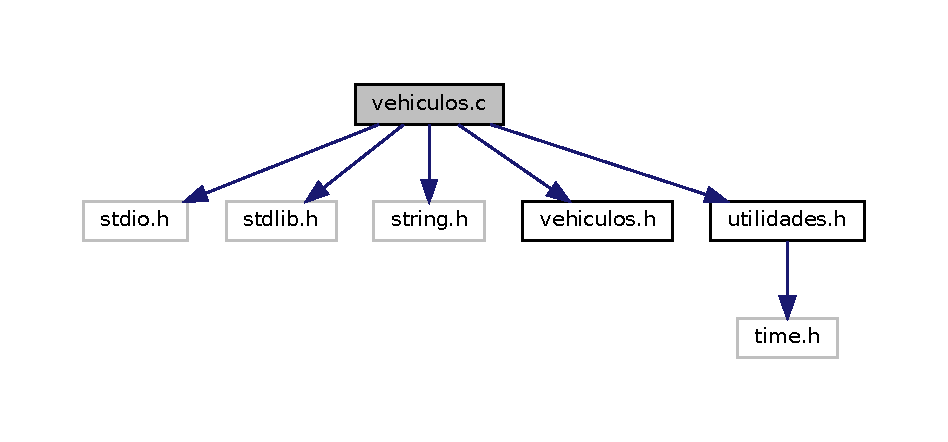
\includegraphics[width=\textwidth, angle=0,scale=0.9]{dep/vehiculos_include.pdf}
\subsection{Estructura de Datos}
\begin{itemize}
    \item \funrf{struct Vehiculos}{struct:vehiculos}
    \item \funrf{struct vVehiculos}{struct:vvehiculos}
\end{itemize}
\subsection{Funciones}
\begin{itemize}
    \item \cc{Vehiculos* initVehiculos(int* n)}
    \item \cc{void saveVehiculos(int n ,Vehiculos* vehiculos)}
    \item \cc{int buscarIndexVehiculo(vVehiculos* v,char* mat)}
    \item \cc{void altaVehiculos(vVehiculos* v,int userId)}
    \item \cc{void listarVehiculos(vVehiculos* v)}
    \item \cc{int* listarVehiculosViajes(vVehiculos* v,int id_user,int *j)}
    \item \cc{void listarVehiculosUser(vVehiculos* v,int userId)}
    \item \cc{void eliminarVehiculoUser(vVehiculos* v,int userId)}
    \item \cc{void modificarVehiculoUser(vVehiculos* v,int userId)}
    \item \cc{void altaVehiculosAdmin(vVehiculos* v)}
    \item \cc{void bajaVehiculosAdmin(vVehiculos* v)}
    \item \cc{void modificarVehiculosAdmin(vVehiculos* v)}
\end{itemize}
\subsection{Definiciones}
\begin{itemize}
	\item \cc{Vehiculos* initVehiculos(int* n)}
	\begin{itemize}
		\item \textbf{Descripcion}
        \begin{itemize}
			\item Inicializa los vehículos.
		\end{itemize}
        \item \textbf{Parametros}
		\begin{itemize}
			\item \cc{n} $\rightarrow$ Índice.
		\end{itemize}
		\item \textbf{Devuelve}
		\begin{itemize}
			\item Vehículos inicializados
		\end{itemize}
	\end{itemize}
	\item\cc{void saveVehiculos(int n ,Vehiculos* vehiculos)}
	\begin{itemize}
		\item \textbf{Descripcion}
        \begin{itemize}
			\item Guarda los vehículos.
		\end{itemize}
        \item \textbf{Parametros}
		\begin{itemize}
			\item \cc{n} $\rightarrow$ Índice.
            \item \cc{vehiculos} $\rightarrow$ Estructura.
		\end{itemize}
	\end{itemize}
    \item\cc{int buscarIndexVehiculo(vVehiculos* v,char* mat)}
	\begin{itemize}
		\item \textbf{Descripcion}
        \begin{itemize}
			\item Busca el índice o identificador del vehículo en cuestión en el vector vehículos.
		\end{itemize}
        \item \textbf{Parametros}
		\begin{itemize}
			\item \cc{v} $\rightarrow$ Vector vehículos.
            \item \cc{mat} $\rightarrow$ Matrícula del vehículo con el que se está trabajando.
		\end{itemize}
        \item \textbf{Devuelve}
		\begin{itemize}
			\item \cc{nose} $\rightarrow$ Índice en el vector vehiculos del vehículo buscado.
		\end{itemize}
	\end{itemize}
    \item\cc{void altaVehiculos(vVehiculos* v,int userId)}
	\begin{itemize}
		\item \textbf{Descripcion}
        \begin{itemize}
			\item Da de alta el vehículo deseado.
		\end{itemize}
        \item \textbf{Parametros}
		\begin{itemize}
			\item \cc{v} $\rightarrow$ Vector vehiculos.
            \item \cc{userId} $\rightarrow$ Identificador del usuario logueado.
		\end{itemize}
	\end{itemize}
	\item\cc{void listarVehiculos(vVehiculos* v)}
	\begin{itemize}
		\item \textbf{Descripcion}
        \begin{itemize}
			\item Lista los vehículos cuando se le llama.
		\end{itemize}
        \item \textbf{Parametros}
		\begin{itemize}
			\item \cc{v} $\rightarrow$ Vector vehiculos.
		\end{itemize}
	\end{itemize}
    \item\cc{int* listarVehiculosViajes(vVehiculos* v,int id_user,int *j)}
	\begin{itemize}
		\item \textbf{Descripcion}
        \begin{itemize}
			\item Devuelve los índices de los vehículos que cumplen la condición.
		\end{itemize}
        \item \textbf{Parametros}
		\begin{itemize}
			\item \cc{v} $\rightarrow$ Vector vehiculos.
            \item \cc{id_user} $\rightarrow$ Identificador del usuario logueado.
            \item \cc{j} $\rightarrow$ Índice viajes.
		\end{itemize}
        \item \textbf{Devuelve}
		\begin{itemize}
			\item \cc{nose} $\rightarrow$ Índice del vehículo que cumple la condición.
		\end{itemize}
	\end{itemize}
    \item\cc{void listarVehiculosUser(vVehiculos* v,int userId)}
	\begin{itemize}
		\item \textbf{Descripcion}
        \begin{itemize}
			\item Función de usuario para el listado de los vehículos que posee.
		\end{itemize}
        \item \textbf{Parametros}
		\begin{itemize}
			\item \cc{v} $\rightarrow$ Vector vehiculos.
            \item \cc{userId} $\rightarrow$ Identificador del usuario logueado.
		\end{itemize}
	\end{itemize}
    \newpage
    \item\cc{void eliminarVehiculoUser(vVehiculos* v,int userId)}
	\begin{itemize}
		\item \textbf{Descripcion}
        \begin{itemize}
			\item Función de usuario para el borrado de los vehiculos que posee.
		\end{itemize}
        \item \textbf{Parametros}
		\begin{itemize}
			\item \cc{v} $\rightarrow$ Vector vehiculos.
            \item \cc{userId} $\rightarrow$ Identificador del usuario logueado.
		\end{itemize}
	\end{itemize}
   \item\cc{void modificarVehiculoUser(vVehiculos* v,int userId)}
	\begin{itemize}
		\item \textbf{Descripcion}
        \begin{itemize}
			\item Función de usuario para la modificación de los vehículos que posee.
		\end{itemize}
        \item \textbf{Parametros}
		\begin{itemize}
			\item \cc{v} $\rightarrow$ Vector vehiculos.
            \item \cc{userId} $\rightarrow$ Identificador del usuario logueado.
		\end{itemize}
	\end{itemize}
    \item\cc{void altaVehiculosAdmin(vVehiculos* v)}
	\begin{itemize}
		\item \textbf{Descripcion}
        \begin{itemize}
			\item Función de administrador para el alta de vehículos en la base de datos.
		\end{itemize}
        \item \textbf{Parametros}
		\begin{itemize}
			\item \cc{v} $\rightarrow$ Vector vehiculos.
         	\end{itemize}
	\end{itemize}
    \item\cc{void bajaVehiculosAdmin(vVehiculos* v)}
	\begin{itemize}
		\item \textbf{Descripcion}
        \begin{itemize}
			\item Función de administrador para la eliminación de vehículos de la base de datos.
		\end{itemize}
        \item \textbf{Parametros}
		\begin{itemize}
			\item \cc{v} $\rightarrow$ Vector vehiculos.
         	\end{itemize}
	\end{itemize}
    \item\cc{void modificarVehiculosAdmin(vVehiculos* v)}
	\begin{itemize}
		\item \textbf{Descripcion}
        \begin{itemize}
			\item Función de administrador para la edición de los vehículos de la base de datos.
		\end{itemize}
        \item \textbf{Parametros}
		\begin{itemize}
			\item \cc{v} $\rightarrow$ Vector vehiculos.
         	\end{itemize}
	\end{itemize}

\end{itemize}
\newpage
